\documentclass[../main.tex]{subfiles}

\begin{document}
\begin{problema}
	Un atleta está parado en la cima de una montaña cuya pendiente hace
	un ángulo \(\phi\) en la horizontal, como se muestra en la figura.
	¿A qué ángulo \(\theta\) debe lanzar una pelota de manera
	que el alcance sea máximo?

	\begin{figure}[htp]
		\centering
		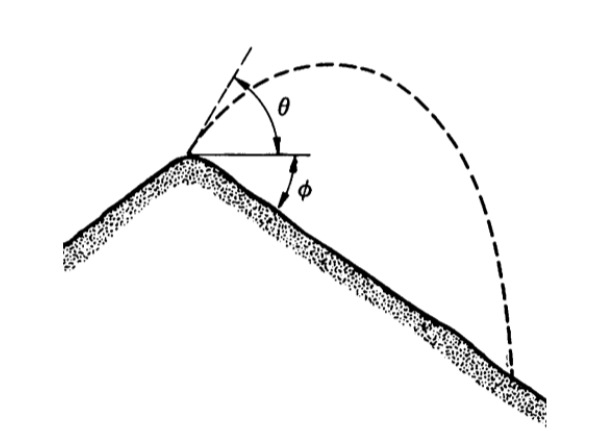
\includegraphics[scale=.4,trim={2cm 1cm 1.2cm 1.2cm}, clip]{../figs/problema_02.jpg}
	\end{figure}

	\startsolution

	Nos encontramos en presencia de un movimiento parabólico, del que sabemos
	tenemos movimiento constante en la dirección horizontal y aceleración constante,
	\(\va{a} = (0, -g)\), en la dirección vertical. Sin embargo, esto es válido si
	nuestro sistema de referencia está en la cima de la montaña. Es por ello que si
	ahora colocamos nuestro sistema de referencia en la pendiente de la montaña, el
	ángulo que nos interesa es

	\begin{equation*}
		\alpha = \theta - \phi.
	\end{equation*}

	Y, además,

	\begin{equation*}
		a_{x} = g\sin\phi,\qquad a_{y} = -g\cos\phi.
	\end{equation*}

	Mientras que las componentes de la velocidad son

	\begin{align*}
		v_{xi} & = v_{i}\cos\alpha, \\
		v_{yi} & = v_{i}\sin\alpha.
	\end{align*}

	Nos interesa encontrar el punto en el que \(y = 0\), para lo que
	determinamos el tiempo que le toma alcanzar la altura máxima, i.e.
	\(v_{y} = 0\). Entonces,

	\begin{align}
		0             & = v_{i}\sin\alpha - g\cos\phi,\nonumber                 \\
		g\cos(\phi) t & = v_{i}\sen\alpha,\nonumber                             \\
		t             & = \dfrac{2v_{i}\sen\alpha}{g\cos\theta}.\label{eq:time}
	\end{align}

	Multiplicando por 2 la \zcref{eq:time} obtenemos el
	tiempo total de vuelo,

	\begin{equation}
		t = \dfrac{2v_{i}\sin\alpha}{g\cos\phi}.
		\label{eq:tTotal}
	\end{equation}

	Para encontrar la posición en función del ángulo, sustituimos la
	\zcref{eq:tTotal} en la expresión \(x = x_{0} + v_{xi}t + \tfrac{1}{2}a t^{2}\),

	\begin{align}
		x & = v_{i}\cos\alpha \Biggl(\dfrac{2v_{i}\sen\alpha}{g\cos\phi}\Biggr) +
		\dfrac{1}{2}(g\sin\phi)\Biggl(\dfrac{2v_{i}\sin\alpha}{g\cos\phi}\Biggr),\nonumber \\
		  & = \dfrac{2v_{i}^{2}}{g}\Biggl[\dfrac{\sin(2\alpha)}{2\cos\phi} +
			\dfrac{\sin\phi\sin^{2}\alpha}{g\cos^{2}\phi}\Biggr].
		\label{eq:xAlpha}
	\end{align}

	Derivamos la \zcref{eq:xAlpha} como primer paso para
	encontrar el ángulo máximo,

	\begin{align*}
		\odv{x}{\alpha} & = \dfrac{2v_{i}^{2}}{g}\Biggl[\dfrac{2\cos 2\alpha}{2\cos\phi} + \dfrac{\sin\phi}{\cos^{2}\phi}2\cos\alpha\sin\alpha\Biggr], \\
		                & = \dfrac{2v_{i}^{2}}{g}\Biggl[\dfrac{\cos 2\alpha\cos\phi + \sen\phi\sin 2\alpha}{\cos^{2}\phi}\Biggr].
	\end{align*}

	Pero esto se parece a la identidad trigonométrica \(\cos(\phi - 2\alpha)\),

	\begin{equation}
		\odv{x}{\alpha} = \dfrac{2v_{i}^{2}}{g}\dfrac{\cos(\phi - 2\alpha)}{\cos^{2}\phi}.
		\label{eq:dvX}
	\end{equation}

	Igualamos la \zcref{eq:dvX} a cero,

	\begin{align*}
		0 & = \dfrac{2v_{i}^{2}}{gcos^{2}\phi}\cos(\phi - 2\alpha), \\
		0 & = \cos(\phi - 2\alpha).
	\end{align*}

	Pero los ceros de cosenos se encuentran en

	\begin{align*}
		\phi - 2\alpha          & = \dfrac{(2n + 1)\pi}{2},\qquad n = 0,1,\dots \\
		\phi - 2(\theta - \phi) & = \dfrac{(2n + 1)\pi}{2},                     \\
		2\theta - \phi          & = \dfrac{(2n + 1)\pi}{2},                     \\
		\theta                  & = \dfrac{(2n + 1)\pi}{4} + \dfrac{\phi}{2}.
	\end{align*}

	En particular, como \(\phi, \theta < \tfrac{\pi}{2}\) nos tomamos \(n = 0\),

	\begin{empheq}[box=\mainresult]{equation*}
		\theta = \dfrac{\pi}{4} + \dfrac{\phi}{2}.
	\end{empheq}
\end{problema}
\end{document}
